\chapter{Evaluación del Sistema}
\label{ch:evaluacion}

\section{Estrategia de evaluación}

Evaluar un sistema construido sobre \ac{LLM} plantea una dificultad propia: sus componentes no
son deterministas —una misma entrada puede producir salidas distintas entre ejecuciones— y sus
fallos son silenciosos, pues una alucinación tiene la misma forma que una extracción correcta.
Sin una medición sistemática y repetible es imposible saber si un cambio de \textit{prompt}, de
modelo o de umbral mejora el sistema o lo degrada. La estrategia de evaluación de \textbf{Seshat}
responde a esa dificultad con dos decisiones: medir por separado cada etapa no determinista, y
convertir el resultado de esa medición en una condición de despliegue.

La calidad se mide con cinco arneses independientes, uno por cada etapa del \textit{pipeline} con
comportamiento no determinista: identificación, agrupación, \textit{grounding}, recuperación
(\textit{retrieval}) y resolución de relaciones. La elección de esas cinco etapas no es arbitraria:
el resto del \textit{pipeline}  es determinista y queda cubierto por las pruebas unitarias y de
integración habituales, donde una salida incorrecta delata un error de código. Sólo estas cinco
etapas, cuya salida depende de un \ac{LLM} o de la similitud vectorial, pueden degradarse en
silencio ante un cambio de \textit{prompt}, de modelo o de corpus, sin que ninguna prueba
convencional lo advierta; por eso son las que exigen medirse contra una referencia.

Cada arnés ejecuta el componente real del sistema contra un corpus de casos con verdad de referencia,
y produce métricas de precisión y \textit{recall} adaptadas a la tarea que evalúa, calculadas por
\textit{scorers} deterministas propios y no por un LLM como juez, para que el veredicto sea
reproducible. Lo que se mide es así exactamente lo que se ejecuta en producción. Aislar cada etapa
cumple además un segundo
propósito, más allá de la cobertura: atribuir una regresión a su origen. Como la resolución opera
sobre los candidatos que le entrega la recuperación, un fallo observado de principio a fin podría
nacer en cualquiera de las dos; medirlas por separado, cada una contra su propia verdad de referencia,
distingue si el problema está en \emph{qué} se recuperó o en \emph{cómo} se clasificó.

Los cinco arneses vuelcan su veredicto —una métrica por criterio, con su marca de aprobado o
suspenso— a un fichero de \textit{gate} común que agrega los resultados de todos los arneses
ejecutados. Ese fichero no es un mero informe: la \ac{API} se niega a arrancar si el \textit{gate}
no está presente o no ha pasado, de manera que el sistema no puede procesar datos reales con
una calidad por debajo de los objetivos fijados. Los umbrales que definen ese aprobado residen
en código, no en configuración, para que modificarlos exija un cambio revisable y no un simple
ajuste de entorno.

La tabla~\ref{tab:eval-gate-criteria} recoge el contrato completo de calidad: qué mide cada arnés,
qué umbral debe superar cada métrica para aprobar y si su incumplimiento bloquea el arranque del
sistema. No todas las métricas medidas condicionan el \textit{gate}: algunas se registran en
MLflow solo con fines de observabilidad, pues resultan demasiado estrictas o poco discriminantes
para servir de criterio de bloqueo —una distinción que se justifica caso por caso en los
resultados de cada arnés.

\begin{table}[htbp]
  \centering
  \small
  \setlength{\tabcolsep}{12pt}
  \begin{tabular}{l l l l}
    \toprule
    \textbf{Arnés} & \textbf{Métrica} & \textbf{Umbral} & \textbf{Bloqueante} \\
    \midrule
    Identificación & precisión (por tipo)  & $\geq$0.75--0.85 & Sí \\
                   & recall (por tipo)     & $\geq$0.75--0.85 & Sí \\
                   & tasa espuria (por tipo) & $\leq$0.10--0.15 & Sí \\
                   & F1                    & ---              & No \\
    \addlinespace
    \cmidrule[0.02em]{1-4}
    Agrupación & \texttt{group\_hit\_rate} & $\geq$0.80 & Sí \\
               & \texttt{exact\_match}     & ---        & No \\
    \addlinespace
    \cmidrule[0.02em]{1-4}
    \textit{Grounding} & precisión & $\geq$0.85 & Sí \\
                       & recall    & $\geq$0.80 & Sí \\
    \addlinespace
    \cmidrule[0.02em]{1-4}
    Recuperación & \texttt{recall@5}    & $\geq$0.70 & Sí \\
                 & \texttt{mrr@5}       & $\geq$0.75 & Sí \\
                 & \texttt{precision@5} & ---        & No \\
    \addlinespace
    \cmidrule[0.02em]{1-4}
    Resolución & precisión (por tipo) & $\geq$0.80 & Sí \\
               & recall (por tipo)    & $\geq$0.80 & Sí \\
               & F1                   & ---        & No \\
    \bottomrule
  \end{tabular}
  \caption{Criterios del \textit{gate} de evaluación: métricas medidas por cada arnés, umbral de
           aprobado y si su incumplimiento impide el arranque del sistema. Los umbrales de
           identificación varían según el tipo de concepto; se indica su rango y los valores
           exactos por tipo se recogen en la tabla~\ref{tab:eval-identification}.}
  \label{tab:eval-gate-criteria}
\end{table}

La arquitectura interna de los arneses —el emparejador \textit{greedy} de identificación, el
mecanismo de caché compartido y el diseño de las trazas de MLflow— se detalla en el
anexo~\ref{anx:harnesses-eval}; este capítulo se centra en qué se mide, con qué corpus y con qué
resultado.

\section{Corpus sintético de evaluación}

En ausencia de transcripciones reales de reuniones —por razones de privacidad y disponibilidad—
el corpus de referencia se genera con apoyo de un LLM: cada fichero YAML describe un escenario
de reunión sintético junto con la salida esperada del componente bajo prueba. Un corpus
curado a partir de datos reales sería preferible, pero no es viable en esta fase del proyecto.
A pesar de ello, todos los casos se diseñan y revisan manualmente para compensar parcialmente
esta limitación.

Cada arnés organiza su corpus en \textit{tiers}: familias de casos que comparten un mismo
propósito de prueba y cuyo nombre de fichero lleva el \textit{tier} como prefijo explícito,
seguido de un número de secuencia y de una descripción breve del escenario. Así, un fichero
como \texttt{boundary\_001\_decision\_coexists\_with\_risk.yaml} revela sin abrirlo tanto su
rol como la ambigüedad que ejercita: una decisión y un riesgo que conviven en el mismo fragmento.
Esta convención permite auditar de un vistazo la cobertura del corpus y añadir casos nuevos
sin romper su organización. La tabla~\ref{tab:eval-corpus} resume la composición actual:

\begin{table}[htbp]
  \centering
  \small
  \begin{tabularx}{\textwidth}{l >{\raggedright\arraybackslash}X r}
    \toprule
    \textbf{Tier} & \textbf{Rol del caso} & \textbf{Casos} \\
    \midrule
    \multicolumn{2}{l}{\textbf{Identificación}} & \textbf{31} \\
    \cmidrule[0.02em]{1-3}
    \texttt{happy}       & Transcripciones claras y cooperativas; la extracción debe acertar con alta confianza & 10 \\
    \texttt{boundary}    & Interacciones entre tipos donde el agente tiende a alucinar o a suprimir de más & 8 \\
    \texttt{negative}    & Uno o más agentes deben devolver vacío; ejercita los criterios de rechazo & 7 \\
    \texttt{adversarial} & Trampas de inyección de \textit{prompt} y de atribución de responsable & 3 \\
    \texttt{realistic}   & Transcripciones largas y naturales, con deriva temática y varios locutores & 3 \\
    \addlinespace
    \multicolumn{2}{l}{\textbf{Resolución}} & \textbf{44} \\
    \cmidrule[0.02em]{1-3}
    \texttt{simple}    & Un nodo fuente y uno de la base: una única relación esperada evidente, o ninguna & 23 \\
    \texttt{null}      & Salida esperada sin relaciones; nodos temáticamente próximos pero no vinculados & 11 \\
    \texttt{multi}     & Un nodo fuente frente a varios candidatos; algunos relacionados, otros no & 7 \\
    \texttt{realistic} & Contexto completo de reunión: varios nodos fuente y de la base, mezcla de tipos & 3 \\
    \addlinespace
    \multicolumn{2}{l}{\textbf{Recuperación}} & \textbf{40} \\
    \cmidrule[0.02em]{1-3}
    \texttt{same\_type}  & \textit{Pool} de un solo tipo; consulta y candidato del mismo tipo & 4 \\
    \texttt{cross\_type} & \textit{Pool} de un solo tipo; consulta y candidato de tipos distintos & 9 \\
    \texttt{realistic}   & \textit{Pool} mixto de los cuatro tipos; distribución realista de producción & 17 \\
    \texttt{negative}    & \textit{Pool} mixto sin candidatos relevantes; nada debería situarse arriba & 10 \\
    \addlinespace
    \multicolumn{2}{l}{\textbf{Agrupación}} & \textbf{8} \\
    \cmidrule[0.02em]{1-3}
    \texttt{singleton} & Cada ítem debe formar su propio grupo; no hay fusión & 2 \\
    \texttt{merge}     & Varios ítems que deben fundirse en un único grupo & 2 \\
    \texttt{mixed}     & Combinación de ítems que se fusionan y de ítems que quedan sueltos & 2 \\
    \texttt{realistic} & Transcripciones largas; agrupación de extremo a extremo & 2 \\
    \addlinespace
    \multicolumn{2}{l}{\textbf{\textit{Grounding}}} & \textbf{12} \\
    \cmidrule[0.02em]{1-3}
    \texttt{faithful}      & La cita respalda genuinamente la afirmación; el agente no debe rechazar de más & 5 \\
    \texttt{hallucination} & La afirmación añade hechos ausentes en la cita; el agente debe detectar la fabricación & 6 \\
    \texttt{adversarial}   & Trampas de inyección de \textit{prompt} y de manipulación de identidad & 1 \\
    \bottomrule
  \end{tabularx}
  \caption{Composición del corpus de evaluación por arnés y \textit{tier}, con el rol que cumple
           cada \textit{tier} y su número de casos.}
  \label{tab:eval-corpus}
\end{table}

Los \textit{tiers} \texttt{negative} y \texttt{null} merecen una mención aparte: comprueban que
el sistema no extrae ni resuelve nada cuando no corresponde, un aspecto que la precisión sólo
capta indirectamente. Los \texttt{boundary} y \texttt{adversarial}, por su parte, documentan
dentro del propio fichero por qué un caso es ambiguo; esa nota sobrevive a los cambios de
\textit{prompt} y evita que una simple oscilación de puntuación se confunda con una regresión
real.

\section{Métricas y resultados por arnés}

Los resultados de esta sección corresponden a la última ejecución del \textit{gate} sobre el
corpus descrito (\texttt{eval\_gate.json}). Las tablas recogen los valores medidos; el umbral que
cada métrica debe superar y su carácter bloqueante figuran en el contrato de la
tabla~\ref{tab:eval-gate-criteria}. En identificación, cuyos umbrales varían por tipo de concepto,
se repiten junto a cada valor para facilitar la comparación directa.

Todos los arneses puntúan con \textit{scorers} deterministas propios, sin recurrir a un LLM como
juez: solapamiento difuso de citas y campos en identificación, comparación de conjuntos en
agrupación, matrices de confusión en \textit{grounding}, métricas de posición en \textit{retrieval}
y coincidencia exacta de ternas en resolución. La decisión es deliberada. Un juez basado en LLM
reintroduciría en la propia medición el no determinismo y potenciales alucinaciones, y volvería el
veredicto irreproducible; un \textit{scorer} determinista, en cambio, produce la misma puntuación
ante la misma predicción.

El no determinismo residual proviene entonces del \textit{pipeline} evaluado, no del instrumento de
medida: incluso a temperatura cero, la salida del \ac{LLM} puede variar entre ejecuciones por la
no asociatividad de la aritmética en coma flotante bajo ejecución en
paralelo~\cite{goldberg1991floating}. Que el instrumento sea determinista es condición necesaria
para que ese ruido no se confunda con el del sistema, para que el \textit{gate} sea un criterio
estable y para el requisito de evaluación funcionalmente determinista del
capítulo~\ref{ch:requisitos-diseno}.

\subsection{Identificación}

El arnés de identificación ejecuta la primera pasada de extracción sobre la transcripción de cada
caso y empareja los nodos extraídos con los esperados para contarlos como aciertos, falsos
positivos o falsos negativos; el emparejador que decide esas correspondencias se describe en el
anexo~\ref{anx:harnesses-eval}. De ese recuento salen la precisión y el \textit{recall} por tipo
de concepto. Junto a ellos se registra la \textbf{tasa espuria}, que mide un fallo distinto: la
extracción de un tipo de concepto que no debería aparecer en el caso. Se calcula sobre los casos
donde un tipo está ausente de la verdad de referencia, como la fracción de ellos en los que el
agente extrajo al menos un nodo de ese tipo; captura así la contaminación entre tipos que la
precisión, calculada por tipo, no refleja.

\begin{table}[H]
  \centering
  \begin{tabular}{lccc}
    \toprule
    \textbf{Tipo} & \textbf{Precisión} & \textbf{Recall} & \textbf{Tasa espuria} \\
    \midrule
    \texttt{decision}      & 0.964 ($\geq$0.80) & 0.893 ($\geq$0.80) & 0.000 ($\leq$0.10) \\
    \texttt{risk}          & 0.850 ($\geq$0.75) & 1.000 ($\geq$0.80) & 0.000 ($\leq$0.10) \\
    \texttt{action\_item}  & 0.895 ($\geq$0.85) & 0.947 ($\geq$0.85) & 0.077 ($\leq$0.10) \\
    \texttt{open\_question}& 0.867 ($\geq$0.75) & 0.867 ($\geq$0.75) & 0.111 ($\leq$0.15) \\
    \bottomrule
  \end{tabular}
  \caption{Precisión, recall y tasa espuria de identificación por tipo de concepto. Cada valor
           está promediado sobre los casos del corpus.}
  \label{tab:eval-identification}
\end{table}

Los cuatro tipos superan su umbral. El umbral de tasa espuria de \texttt{open\_question} es
deliberadamente más laxo (0.15 frente a 0.10): la frontera entre una pregunta abierta y un
riesgo o una decisión pendiente es genuinamente ambigua en el lenguaje conversacional, y así
queda reflejado también en su tasa espuria observada, la más alta de los cuatro tipos.

\subsection{Agrupación}

La agrupación es el paso que consolida las decisiones fragmentadas de la primera pasada en un
único nodo por decisión (sección~\ref{sec:agentes-identificacion}). El agente recibe la lista
plana de conceptos extraídos y la reparte en grupos, cada uno destinado a fundirse en un solo
nodo, de manera que su salida es una partición $P$ de esos conceptos que se contrasta con la
partición de referencia $E$. Ambas se tratan como conjuntos de grupos, y cada grupo como un
conjunto de conceptos, por lo que ni el orden de los grupos ni el de los conceptos dentro de
cada grupo influye en la puntuación. Sobre ellas se definen dos métricas, que comparan las
particiones a distinta resolución:

\begin{equation}
  \text{exact\_match} =
  \begin{cases}
    1 & \text{si } P = E, \\
    0 & \text{en caso contrario,}
  \end{cases}
  \qquad
  \text{group\_hit\_rate} = \frac{\lvert P \cap E \rvert}{\lvert E \rvert}.
\end{equation}

La primera es una medida de todo o nada: vale 1 sólo si la partición predicha coincide íntegramente
con la esperada y cae a 0 en cuanto un solo grupo difiere. La segunda concede crédito parcial: es la
fracción de grupos esperados que reaparecen exactamente en la predicción.

\begin{table}[H]
  \centering
  \begin{tabular}{lc}
    \toprule
    \textbf{Métrica} & \textbf{Valor} \\
    \midrule
    \texttt{exact\_match}    & 0.750 \\
    \texttt{group\_hit\_rate}& 0.850 \\
    \bottomrule
  \end{tabular}
  \caption{Resultados del arnés de agrupación. Cada valor está promediado sobre los casos del
           corpus.}
  \label{tab:eval-grouping}
\end{table}

Sólo \texttt{group\_hit\_rate} condiciona el \textit{gate}; \texttt{exact\_match} se registra pero
no bloquea, por ser demasiado estricta a medida que crece el número de grupos por caso: un único
grupo mal formado hunde toda la puntuación del ejemplo aunque el resto sea correcto. La brecha entre
ambos valores observados —0.750 frente a 0.850— es precisamente esa penalización: el agente acierta
la mayoría de los grupos, pero rara vez reproduce la partición entera sin un solo desajuste, y es
\texttt{group\_hit\_rate} quien recoge ese acierto parcial que \texttt{exact\_match} descarta.

\subsection{Grounding}

El \textit{grounding} es la compuerta opcional que, durante la puntuación de confianza, verifica
si la cita de un nodo respalda su título y descripción
(sección~\ref{sec:confidence-scoring}). Su arnés mide si el agente emite ese juicio correctamente:
cada nodo del corpus lleva anotado si su cita lo respalda o no, y la predicción del agente se
clasifica en la matriz de confusión (verdaderos y falsos positivos y negativos) que se agrega en
precisión y \textit{recall}.

\begin{table}[H]
  \centering
  \begin{tabular}{lc}
    \toprule
    \textbf{Métrica} & \textbf{Valor} \\
    \midrule
    Precisión & 1.000 \\
    Recall    & 1.000 \\
    \bottomrule
  \end{tabular}
  \caption{Resultados del arnés de \textit{grounding}. Ambos valores se agregan sobre todos los
           nodos del corpus en una única matriz de confusión.}
  \label{tab:eval-grounding}
\end{table}

El resultado perfecto debe leerse con cautela: el corpus de \textit{grounding} es de los más pequeños
de los cinco (12 casos), de modo que el 1.000 significa «sin fallos observados en 12 casos», no una
garantía de perfección; un único caso adicional podría desplazar la métrica de forma apreciable.

\subsection{Recuperación (retrieval)}

Los tres arneses anteriores cubren la primera pasada de extracción; los dos siguientes evalúan la
segunda, que arranca recuperando los nodos con los que cada nodo nuevo podría relacionarse
(sección~\ref{sec:rag-resolucion}). El arnés de recuperación siembra el almacén vectorial con los
candidatos de cada caso y comprueba si la búsqueda sitúa los nodos relevantes entre los cinco
primeros resultados.

Es también la etapa más configurable del \textit{pipeline}: el modo de búsqueda, los modelos de
lenguaje de sus patas densa y dispersa —con sus propios parámetros— y el modelo de
\textit{embeddings} son todos intercambiables (sección~\ref{sec:rag-resolucion}), y cada
combinación desplaza el equilibrio entre latencia, coste y calidad. Las cifras de esta sección no
son, por tanto, un techo del componente, sino el resultado de una configuración concreta, elegida
por ofrecer un buen compromiso entre velocidad y rendimiento.

\begin{table}[H]
  \centering
  \begin{tabular}{lc}
    \toprule
    \textbf{Métrica} & \textbf{Valor} \\
    \midrule
    \texttt{recall@5}    & 0.742 \\
    \texttt{precision@5} & 0.560 \\
    \texttt{mrr@5}       & 0.944 \\
    \bottomrule
  \end{tabular}
  \caption{Resultados del arnés de recuperación. Cada valor está promediado sobre los casos del
           corpus.}
  \label{tab:eval-retrieval}
\end{table}

El corpus mezcla deliberadamente candidatos de los cuatro tipos de concepto en un mismo
\textit{pool} para simular la distribución realista de un almacén
vectorial en producción; un \textit{pool} de un solo tipo suprimiría falsos positivos y
produciría una precisión artificialmente alta. Esta elección explica en parte por qué
\texttt{precision@5} es sensiblemente más baja que \texttt{recall@5} y \texttt{mrr@5}: el
sistema puede devolver candidatos plausibles de otro tipo entre los cinco resultados sin que
ello indique un fallo de recuperación del nodo relevante, que \texttt{mrr@5} confirma que
aparece consistentemente en una posición temprana.

\subsection{Resolución de relaciones}

La resolución es el paso final de la segunda pasada: clasifica la relación entre cada nodo nuevo y
los candidatos recuperados. Su arnés ejecuta esa clasificación y compara las relaciones inferidas
con las esperadas exigiendo coincidencia exacta de la terna (nodo origen, nodo destino, tipo de
relación): una relación sólo cuenta como acierto si coinciden los tres elementos. El criterio es
estricto y no gradúa la gravedad del error, pues todos los desaciertos pesan lo mismo. Por ejemplo,
entre las relaciones que un mismo agente puede asignar a un par de decisiones, confundir
\texttt{amends} con \texttt{supersedes} es un error leve, ya que ambas describen matices de una
misma sustitución. Pero tomar por \texttt{amends} lo que era \texttt{conflicts\_with} es mucho más
grave, ya que invierte la compatibilidad entre ambas decisiones: dar por matización armónica lo que
en realidad es una contradicción activa entre ellas.

Para medir la resolución de forma aislada, el corpus fija a mano el conjunto de candidatos
de cada caso en lugar de tomarlo de la recuperación real: el arnés evalúa así la decisión de
resolución suponiendo una recuperación perfecta, no la calidad de principio a fin.

\begin{table}[H]
  \centering
  \begin{tabular}{lcc}
    \toprule
    \textbf{Tipo de origen} & \textbf{Precisión} & \textbf{Recall} \\
    \midrule
    \texttt{decision}       & 0.910 & 0.962 \\
    \texttt{risk}           & 0.944 & 1.000 \\
    \texttt{action\_item}   & 0.889 & 1.000 \\
    \texttt{open\_question} & 1.000 & 1.000 \\
    \bottomrule
  \end{tabular}
  \caption{Precisión y recall de resolución por tipo de concepto origen. Cada valor está
           promediado sobre los casos del corpus.}
  \label{tab:eval-resolution}
\end{table}

Los cuatro tipos de origen superan con holgura el umbral, pero conviene leer estas cifras a la luz
del supuesto anterior: miden la calidad de la decisión de resolución en condiciones ideales de
recuperación, un límite superior que el rendimiento de principio a fin no necesariamente alcanza.

La tabla anterior desglosa el resultado por tipo de concepto origen, pero no es el único corte
posible: los registros agentes de mismo tipo y tipo cruzado (sección~\ref{sec:agentes-resolucion})
son independientes, cada uno con su propio conjunto de \textit{prompts}: mejorar uno no afecta
al otro, así que separar sus resultados permite atribuir un fallo a la familia responsable en lugar
de diluirlo en un promedio conjunto. Un mismo caso del corpus puede combinar relaciones resueltas
por ambos registros, de modo que la tabla~\ref{tab:eval-resolution-same-cross} puntúa a nivel de
relación individual, reprocesando los resultados cacheados del arnés.

\begin{table}[H]
  \centering
  \begin{tabular}{llcc}
    \toprule
    \textbf{Tipo de origen} & \textbf{Familia} & \textbf{Precisión} & \textbf{Recall} \\
    \midrule
    \multirow{2}{*}{\texttt{decision}}       & Mismo tipo   & 0.857 & 0.967 \\
                                              & Tipo cruzado & 0.875 & 0.875 \\
    \multirow{2}{*}{\texttt{risk}}           & Mismo tipo   & 0.917 & 1.000 \\
                                              & Tipo cruzado & 1.000 & 1.000 \\
    \multirow{2}{*}{\texttt{action\_item}}   & Mismo tipo   & 0.879 & 1.000 \\
                                              & Tipo cruzado & 0.667 & 1.000 \\
    \multirow{2}{*}{\texttt{open\_question}} & Mismo tipo   & 1.000 & 1.000 \\
                                              & Tipo cruzado & 1.000 & 1.000 \\
    \bottomrule
  \end{tabular}
  \caption{Precisión y recall de resolución por tipo de concepto origen y familia de agente,
           puntuados a nivel de relación individual según los tipos de concepto de su nodo origen
           y destino.}
  \label{tab:eval-resolution-same-cross}
\end{table}

El desglose confirma que la resolución de tipo cruzado no es intrínsecamente más difícil que la de
mismo tipo pese a tener más pares origen-destino posibles: en tres de los cuatro tipos de origen
—\texttt{risk}, \texttt{action\_item} y \texttt{open\_question}— el recall de tipo cruzado iguala o
supera al de mismo tipo. La única caída notable de recall es \texttt{decision}, que pierde 9~puntos
al pasar de mismo a tipo cruzado. El caso opuesto —\texttt{action\_item} en tipo cruzado, con la
precisión más baja de toda la tabla (0.667) pero recall perfecto— corresponde a muy pocas relaciones
(3~casos): el agente no omite ninguna relación esperada, pero inventa alguna adicional, un patrón
distinto al de \texttt{decision} y consistente con la limitación de la coincidencia exacta de terna
señalada en la sección~\ref{sec:analisis-errores}.

\section{Calibración de umbrales}

Los arneses anteriores miden el sistema con sus umbrales ya fijados, pero esos umbrales no se
eligen a mano. Dos señales continuas del \textit{pipeline} gobiernan decisiones binarias a través
de un corte, y fijar ese corte por intuición sería arbitrario y frágil: la confianza que determina
si un nodo identificado se aprueba automáticamente o se envía a revisión humana, y la puntuación de
similitud que filtra los resultados de \textit{retrieval}. Ambas se calibran mediante un barrido de
umbral contra el corpus de referencia, buscando el valor que optimiza una métrica objetivo. La
calibración cierra así el ciclo con las secciones anteriores: los mismos arneses que miden la
calidad proveen también los datos con los que se ajustan los parámetros que la gobiernan.

Ese barrido es barato porque reutiliza la caché de predicciones de los arneses correspondientes:
recalcular el umbral óptimo recorre en memoria resultados ya calculados, sin repetir ninguna llamada
al LLM (anexo~\ref{anx:cache-eval}). Las dos subsecciones siguientes detallan qué métrica objetivo
guía cada barrido, pues difieren según lo que cada umbral pone en juego.

\subsection{Umbral de confianza (identificación)}

El umbral sobre la puntuación de confianza heurística decide qué nodos identificados se aprueban
sin intervención humana y cuáles se envían a la revisión (\textit{HITL}). Un nodo por debajo del
umbral no se descarta, sino que se encola para revisión: sólo cambia de canal de aprobación. Por eso
F1 no sirve aquí, ya que contaría ese nodo diferido como un falso negativo.

La calibración se guía en cambio por dos magnitudes complementarias, medidas sobre el conjunto de
nodos auto-aprobados: la \textbf{precisión} —qué fracción de ellos eran correctos— y la
\textbf{cobertura} —qué fracción del total de nodos esperados llegan a auto-aprobarse—. Ambas
tiran en sentidos opuestos: subir el umbral aprueba menos nodos pero más fiables, mejorando la
precisión a costa de la cobertura. El barrido resuelve esa tensión eligiendo el umbral $t^\star$ de
mayor cobertura entre los que aún satisfacen una precisión objetivo $p_{\text{obj}}$ (0.95 por
defecto):

\begin{equation}
  t^\star = \operatorname*{arg\,max}_{t}\ \text{cobertura}(t)
  \quad\text{sujeto a}\quad
  \text{precisión}(t) \ge p_{\text{obj}}.
\end{equation}

Si ningún umbral alcanza $p_{\text{obj}}$, se conserva el de mayor precisión. El umbral resultante
gradúa así cuánta carga de revisión se traslada al operador sin comprometer la fiabilidad de lo que
se aprueba solo.

La figura~\ref{fig:pc-curve} muestra el barrido sobre el corpus de identificación y hace visible
esa tensión: al elevar el umbral, la cobertura desciende de forma monótona mientras la precisión
asciende. Con $p_{\text{obj}}=0{,}95$, el umbral seleccionado es $t^\star=0{,}76$ —el de mayor
cobertura (0,60) entre los que superan la precisión objetivo—, marcado en la figura.

\begin{figure}[htbp]
  \centering
  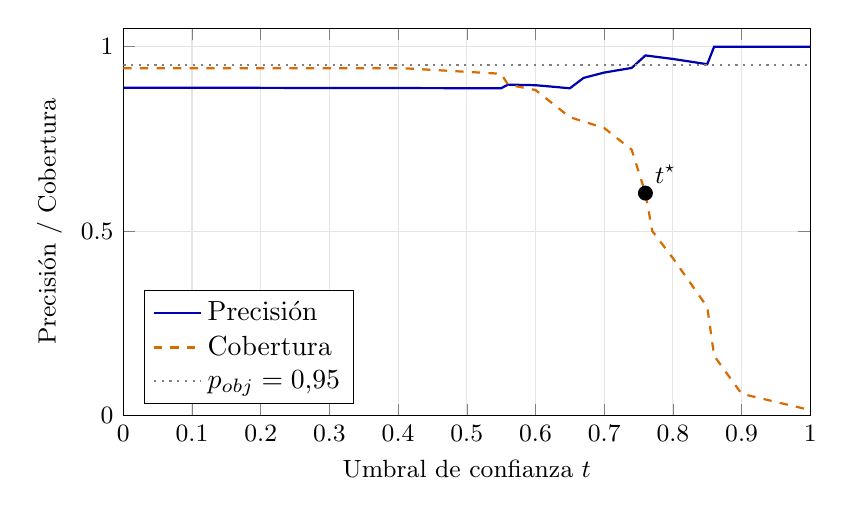
\begin{tikzpicture}
    \begin{axis}[
      width=0.85\textwidth, height=6.5cm,
      xlabel={Umbral de confianza $t$},
      ylabel={Precisión / Cobertura},
      xmin=0, xmax=1, ymin=0, ymax=1.05,
      legend pos=south west,
      legend cell align=left,
      grid=major, grid style={gray!20},
      tick label style={font=\small}, label style={font=\small},
    ]
      \addplot[blue!70!black, thick, mark=none] coordinates {
        (0.00,0.8889) (0.55,0.8873) (0.56,0.8971) (0.60,0.8955) (0.63,0.8906)
        (0.65,0.8871) (0.67,0.9153) (0.70,0.9298) (0.74,0.9423) (0.76,0.9762)
        (0.80,0.9667) (0.85,0.9524) (0.86,1.0000) (0.90,1.0000) (1.00,1.0000)
      };
      \addlegendentry{Precisión}
      \addplot[orange!85!black, thick, dashed, mark=none] coordinates {
        (0.00,0.9412) (0.41,0.9412) (0.55,0.9265) (0.56,0.8971) (0.60,0.8824)
        (0.65,0.8088) (0.70,0.7794) (0.74,0.7206) (0.76,0.6029) (0.77,0.5000)
        (0.80,0.4265) (0.85,0.2941) (0.86,0.1618) (0.90,0.0588) (1.00,0.0147)
      };
      \addlegendentry{Cobertura}
      \addplot[gray, dotted, thick] coordinates {(0,0.95) (1,0.95)};
      \addlegendentry{$p_{\text{obj}}=0{,}95$}
      \addplot[only marks, mark=*, mark size=2.5pt, black] coordinates {(0.76,0.6029)};
      \node[anchor=south west, font=\small] at (axis cs:0.76,0.6029) {$t^\star$};
    \end{axis}
  \end{tikzpicture}
  \caption{Barrido del umbral de confianza sobre el corpus de identificación. La cobertura (fracción
           de nodos auto-aprobados) decrece al subir el umbral, mientras la precisión sobre los
           auto-aprobados crece. El punto $t^\star=0{,}76$ es el de mayor cobertura entre los que
           alcanzan la precisión objetivo $p_{\text{obj}}=0{,}95$.}
  \label{fig:pc-curve}
\end{figure}

La señal que se calibra es puramente heurística. Se contempló complementarla con una segunda señal
basada en \acs{NLI}, que verificara si la descripción de un nodo se deduce de su cita fuente,
pero su incorporación se ha aplazado (capítulo~\ref{ch:conclusiones}): exigiría un modelo adicional
y añadiría latencia por nodo, y queda por confirmar que aporta información realmente ortogonal a las
heurísticas. La calibración opera, por tanto, sobre el único corte heurístico vigente.

\subsection{Umbral de similitud (retrieval)}

El umbral de similitud descarta los candidatos de \textit{retrieval} demasiado poco relevantes
antes de pasarlos a la resolución, y se calibra de forma independiente por modo de búsqueda, ya
que la escala de puntuación no es comparable entre modos: similitud coseno en el modo semántico,
relevancia textual en el de palabras clave y \ac{RRF} en el híbrido. El barrido maximiza el
\textbf{F2 macro-promediado} sobre el corpus: cada caso positivo aporta su F2 —que pondera el
\textit{recall} el doble que la precisión, pues omitir un nodo relevante priva a la resolución de un
candidato válido, un error más costoso que arrastrar uno irrelevante— y cada caso negativo aporta su
especificidad —1 si no devuelve nada por encima del umbral, 0 si cuela algún irrelevante—, de modo
que un umbral degenerado en cero, que lo aceptaría todo, no pueda dominar la selección.

\section{Análisis de errores y limitaciones}
\label{sec:analisis-errores}

Los resultados anteriores deben interpretarse junto con las limitaciones conocidas de cada
arnés:

\begin{itemize}
  \item \textbf{Identificación}: el emparejamiento por solapamiento difuso de citas puede aceptar
        como válida una cita que en realidad pertenece a una frase distinta pero suficientemente
        parecida; además, sólo se puntúan los campos estructurados de cada nodo, no la calidad
        semántica de su título y su descripción.

  \item \textbf{Resolución}: dos limitaciones ya señaladas se combinan —la coincidencia exacta de
        terna no distingue un error grave de uno leve, y el supuesto de recuperación perfecta—, por
        lo que sus cifras son un límite superior optimista.

  \item \textbf{Recuperación}: sólo evalúa la recuperación basada en \textit{embeddings}, pero no el
        efecto del \textit{reranking} posterior y de la expansión por vecinos del grafo.

  \item \textbf{Agrupación y \textit{grounding}}: con 8 y 12 casos son los corpus más pequeños de
        los cinco, lo que limita la confianza estadística de sus métricas frente a los de
        identificación, resolución y recuperación.
\end{itemize}
